\documentclass[a4paper,12pt]{article}
\usepackage{amstext}
\usepackage{rotating}
\usepackage[usenames]{color}
%\usepackage{epsfig}
\usepackage{overpic}
\usepackage{url}
\usepackage{pst-plot}
\usepackage{amsmath,fullpage,graphicx,caption,float}
\usepackage{amssymb}
\usepackage{array,ragged2e,pst-node,pst-dbicons}
\usepackage{pstricks}
\usepackage{pst-node}
\usepackage{pst-blur}
\usepackage{comment}
\usepackage{color}
\usepackage{subfigure}
\usepackage{lscape}
\usepackage{multirow}
\usepackage{hyperref}
\usepackage{mathtools}
\usepackage{framed}
\usepackage{diagbox}

\newcommand{\defeq}{\vcentcolon=}

\usepackage{float}
\restylefloat{table}
\usepackage[margin=20mm]{geometry}

\setlength{\parskip}{1.25ex}
\renewcommand\baselinestretch{1.3}
\renewcommand\arraystretch{1.5}

% equation numbering:
\numberwithin{equation}{section}

\mathchardef\mhyphen="2D
\definecolor{Pink}{rgb}{1.,0.75,0.8}
\newcolumntype{C}[1]{>{\Centering}p{#1}}
\def\Tab#1{\tabular{C{3cm}}\rule[-5mm]{0pt}{1cm}#1\\\hline
                           ~\\\hline~\endtabular}
\seticonparams{entity}{shadow,fillcolor=black!20,fillstyle=solid,framesep=0pt}

\mathchardef\mhyphen="2D
\usepackage[numbers,sort&compress]{natbib}
\usepackage[nottoc]{tocbibind}

  \textwidth  165mm
  \textheight 215mm
  \topmargin 10mm
  \oddsidemargin  10mm
  \evensidemargin 3mm
\renewcommand{\baselinestretch}{1.}
\sloppy



\textwidth  162mm \textheight 230mm \topmargin 0mm \oddsidemargin
0mm \evensidemargin 0mm

\title{RESPONSE TO COMMENTS AND CORRECTIONS
for Analysis Working Group Round 1}

\begin{document}

\date{}
\maketitle

\begin{center}

G. Fedotov, V. Burkert, R. Gothe, V. Mokeev, Iu. Skorodumina\\[1cm]

CLAS Analysis Review Committee:
Evgeny Golovach, Nicolay Markov (chair), and Daniel Carman
\end{center}

Thank you for your comments, questions and suggestions in your .pdf document.
We list here our responses following your comments: \\

{\bf 1. Provide a "good" run list for  this  analysis  in  the  appendix   denoting  both  full target empty target runs. }\\[0.5cm]

The table with the list of full and empty target runs was included in the beginning of Chapter 2 of the analysis note, and also is shown below.

\begin{table}[htp]
\centering 



\begin{tabular}{|c|c|}

\hline
Full target runs & Empty target runs\\
\hline 
36117--36122, 36125--36129, 36133--36142 & 35124  \\
36144, 36145, 36147--36150, 36152--36154 & 36428  \\
36156, 36158--36160, 36429--36434 & 36495  \\ 
36437,  36441--36447, 36449, 36450 & \\
36452--36454, 36458--36467, 36469 & \\
36473--36478, 36480--36482, 36484--36492 & \\
36497--36503, 36505--36511 & \\
\hline 
\end{tabular}
\caption{\small List of the runs that were used in the analysis.}
\end{table}

\vspace{0.5cm}

{\bf 2. Section 2.1 -- You state that the drift chambers were in the "hardware trigger" for e1e. In my recollection we never employed a level 2 hardware trigger including the drift chambers. Please verify your statement. If e1e actually used a level 2 trigger, then you will need to convince me of its efficiency.  }\\[0.5cm]

We are not sure about "hardware trigger", so most likely you are right. We only wanted to state that on the software level we require electron candidates to give signals in all four detectors by emploing the conditions $DCStat > 0$, $CCStat > 0$, $SCStat > 0$, $ECStat > 0$. The corresponding changes were added into the analysis note.\\[0.5cm]


{\bf 3. Page 6. The bullet at the bottom of the page and Page 7 the bullet at the top of the page. The content of both bullets look quite similar. Should they be combined in one bullet?  }\\[0.5cm]

You are right. These two bullets were merged together (see line 153).\\[0.5cm]

{\bf 4. Section 2.1.1 -- Did you employ an EC fiducial cut to ensure that you did not have shower leakage?}\\[0.5cm]

As far as we remember all coordinates in all detector planes (CC, SC, EC) are calculated from DC track. Outside the DC area there is no magnetic field and  particles move along the straight lines. Therefore, fiducial cut applied in one plane automatically removes edge events in other planes.  Since an additional fiducial cuts in CC plane given by formulae 2.1.9 were already applied, we came to the conclusion that the cuts in EC plane are not necessarily needed.\\[0.5cm]

{\bf 5. Section 2.1.1 -- Can you provide a plot of Ein vs. Eout for your electron sample? Usually folks include an Ein cut to eliminate minimum ionizing pions that sneak through other cuts.}\\[0.5cm]

Please find this plot below (see Fig~\ref{eout_ein}). It is also included in the Section 2.1.1 of the analysis note. As it is seen in this plot the spot in the left bottom corner that corresponds to the pion contamination disappears after final electron id. It seems that additional cut on Ein is not needed.

\begin{figure}
\begin{center} 
\framebox{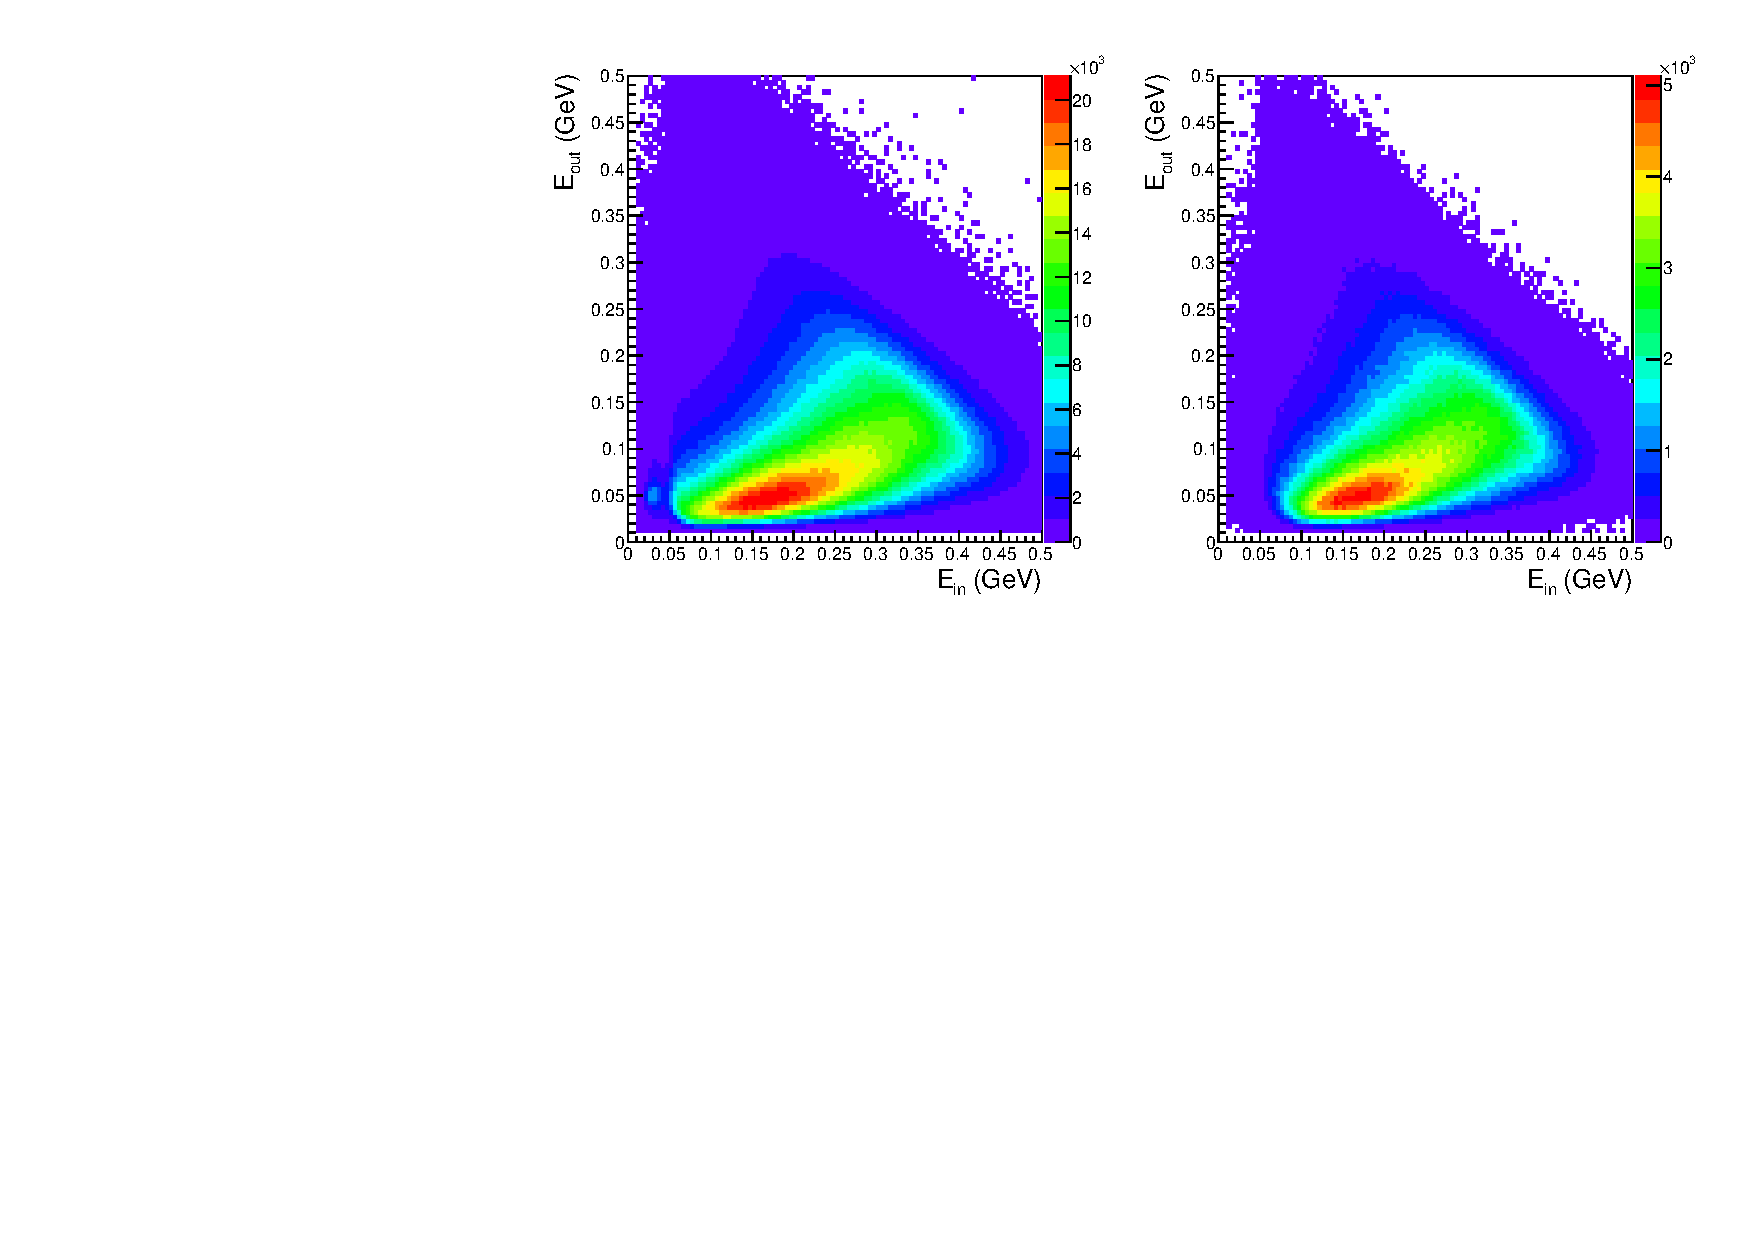
\includegraphics[width=12cm]{eout_vs_ein.pdf}}
\caption{\small Energy deposited in the outer part of EC versus energy deposited in the inner part of EC before (left plot) and after (right plot) electron id. \label{eout_ein}} 
\end{center}
\end{figure}

\vspace{0.5cm}

{\bf 6. Section 2.1.1 -- It is not fully clear from what you have written how you are 
dealing with the CC efficiency.  Fig. 2.4 seems to show an efficiency map but 
apparently you did not use this to correct for the CC trigger inefficiency. 
Instead you used an approach looking at what fell below the single P.E. peak. 
This seems to be a much coarser approach (as Fig. 2.4 has many more pixel 
bins). Please show your efficiencies for the CC and make clear how these 
were included into your cross section extraction. I would like to see 
correspondence between what is shown in Fig. 2.6 with what is shown in Fig. 
2.4.}\\[0.5cm]

In Fig. 2.4 (Fig. 2.5 in the new version) the quantity given by formula 2.1.8 is shown as color code. This quantity is not quite efficiency, it is the portion of good electrons with number of
photoelectrons greater than five inside a ($\theta_{cc}$, $\varphi_{cc}$ ) bin. Geometrical zones ( $\theta_{cc}$, $\varphi_{cc}$ bins) where this ratio is less than 0.8 were removed from the consideration both for the data and MC. So, in other words we applied kind of fiducial cut in the CC plane that removes zones with large amount of bad electron candidates. After this cut had been applied Fig. 2.6 (Fig. 2.7 in the new version) was plotted. After this cut the peak at low number of photoelectrons   significantly decreases, but still remains. So, the standard procedure of eliminating of events with low number of photoelectrons and restoring of portion of good events that were removed was applied. It needs to be mentioned that distributions in Fig. 2.6 (Fig. 2.7 in the new version) were plotted for individual PMTs in each CC segments, so on this way the information about photoelectron distributions was obtained with maximal avaliable detalization level. Moreover the cut shown by the red vertical line in Fig. 2.6 (Fig. 2.7 in the new version) was individually chosen for each of the PMTs. 

The portion of good events shown by blue in Fig. 2.6 (Fig. 2.7 in the new version) was restored by applying a weight factor (given by formula 2.1.12) to each event which goes to the particular PMT. That is why CC efficiency is not explicitly presented as a separate factor in the final cross section formula.

This intricate dealing with CC was elaborated to achieve an agreement of the elastic cross section with the known parameterization. The standard approach that is typically used in many analysises does not allow to achieve this agreement. \\[0.5cm]

{\bf 7. Section 2.1.1  -� If you did use the approach in Fig. 2.6 to account for CC efficiency, how do you deal with regions where there is no hit in the CC? You need a true CC efficiency mapping to make this correction properly.}\\[0.5cm]

The description of the acconting for CC efficiency is given in answer to the question 6. We require each electron candidate to have hit in CC, therefore we are not interested in the regions with no CC hit, since there are no data events to analyze there.\\[0.5cm]

{\bf 8.  Page 12. line 255 What is the reason to choose 5 photoelectrons as a 
criterion of a good electron?}\\[0.5cm] 

This choice was made in order to be sure that the peak at low number of photoelectrons is below this value for most of the PMTs. This choice has no significant influence on the statistics since this value is only used to determine fiducial areas in the CC plane. Moreover this value is better to be greater than smaller since in the numerator of the ratio 2.1.8 it is better to have the number of surely good electron candidates. For different choice of this value one should use correspondingly different value of the cut on ratio 2.1.8 in order to maintain maximum possible statistics. See also the answer to the question six.\\[0.5cm] 

{\bf 9. Page 13. Fig 2.4. Is this plot made with two pion events or with all events? Could you provide the similar plot of the CC efficiency made with the 
simulated two pion events? }\\[0.5cm] 	
    
Plots in Fig. 2.4 (Fig. 2.5 in the new version) are made with inclusive electron candidates. There are no enough two pion events to produce these plots for the purpose of cut establishing. The avaliable two pion statistics does not allow to obtain sufficient population of all bins in the histograms in Fig. 2.4 (Fig. 2.5 in the new version). 

The Fig. 2.4 (Fig. 2.5 in the new version) is used just to determine fiducial areas in the CC plane, but not for the efficiency calculation. It is a common practice to establish fiducial areas basing on the data and applying the cut for both data and MC. This phylosophy was used in this case also.\\[0.5cm]

{\bf 10. Section 2.1.1, Line 261. How do you choose value of the cut to be 0.8? Could 
you make a 1 dimensional plot of CC efficiency for every sector? Do you have 
estimate of what fraction of events you cut out with this cut?}\\[0.5cm]

The plot with one-dimensional slices of Fig. 2.4 (Fig. 2.5 in the new version) is presented below (see Fig.~\ref{cc_eff_one_dimm}). The vertical axis in Fig.~\ref{cc_eff_one_dimm} shows the ratio given by eq. 2.1.8 that in fact is not efficiency (see answer to the question six for more details). The horizontal red line shows the applied cut. As in the case of standard fiducial cuts the condition of ratio  2.1.8 to be greater than 0.8 is chosen in order to select flat areas of the distributions.\\[0.5cm]
	 
\begin{figure}
\begin{center} 
\framebox{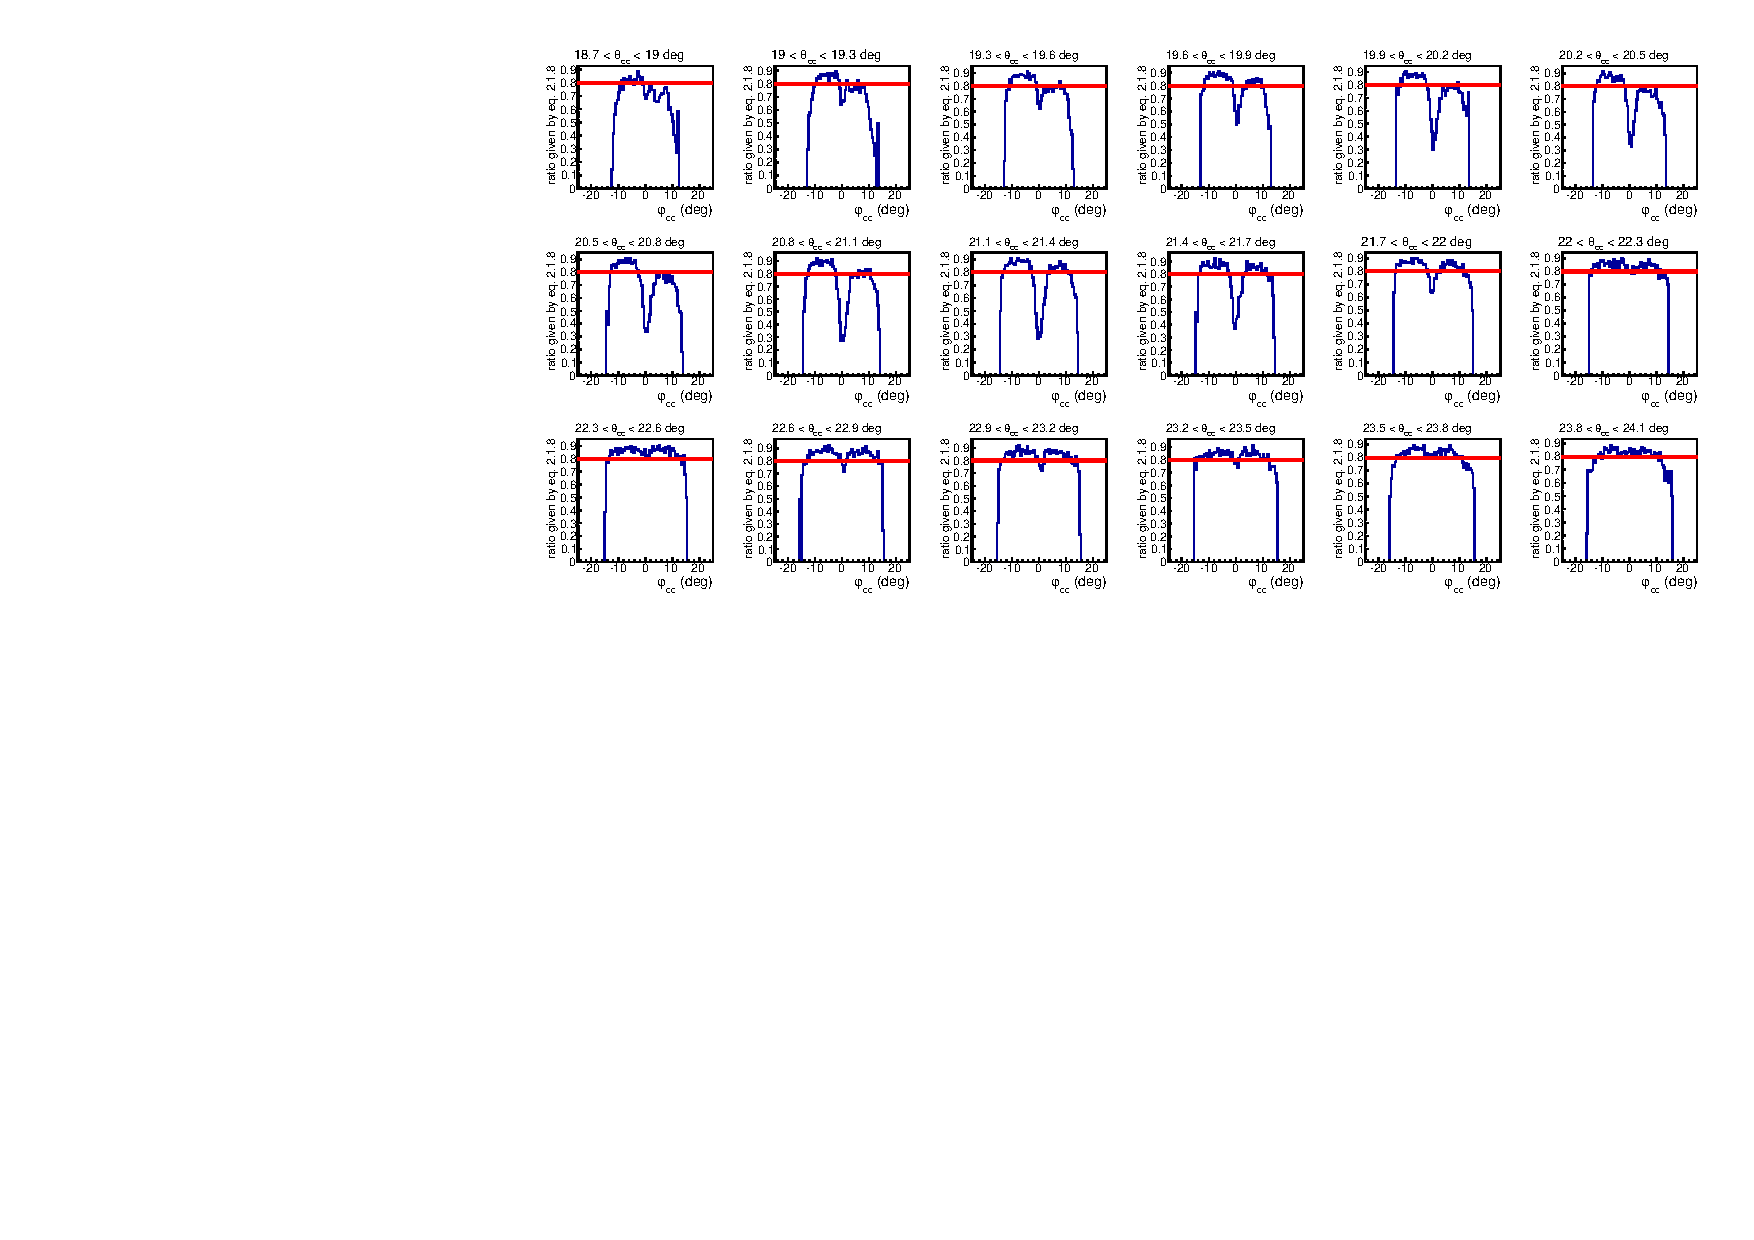
\includegraphics[width=12cm]{cc_eff_one_dimm.pdf}}
\caption{\small One-dimensional slices of the histogram for sector one from Fig. 2.4 (Fig. 2.5 in the new version). Horizontal axis shows $\varphi_{cc}$ while vertical axis shows the ratio given by eq. 2.1.8. The horizontal red line shows the applied cut.   \label{cc_eff_one_dimm}} 
\end{center}
\end{figure}

\vspace{0.5cm}


{\bf 11. Section 2.1.1, Fig. 2.6 What is the typical value of a correction factor?}\\[0.5cm]




The typical value of the correction factor  given by 2.1.12 is 1\%-3\% (see Table~\ref{corr_fact_pmt}).\\[0.5cm]


{\bf 12. Section 2.1.1, Fig. 2.6. Have you tried to look at the efficiency of this cut as functions of other variables, like electron momentum? }\\[0.5cm]	
  
The cuts shown in Fig. 2.6 (Fig. 2.7 in the new version) were applied on the level of individual PMT in each CC segment. These factors for PMTs in sector one are listed in Table~\ref{corr_fact_pmt}. Each CC segment covers relatively narrow range of $\theta$ - angle, so as it seen from Table~\ref{corr_fact_pmt}  the correction factor has no particular angular dependence.   


\begin{table}
\begin{center}
\begin{tabular}{|c|c|}
\hline
Segment number & Correction factor \\
\hline
3 & left PMT - 1.03518, right PMT - 1.03253\\
\hline
4 & left PMT - 1.01850, right PMT - 1.00000\\
\hline
5 & left PMT - 1.01081, right PMT - 1.02871\\
\hline
6 & left PMT - 1.01278, right PMT - 1.04484\\
\hline
7 & left PMT - 1.00533, right PMT - 1.03894\\
\hline
8 & left PMT - 1.00765, right PMT - 1.01455\\
\hline
9 & left PMT - 1.00823, right PMT - 1.00888\\
\hline
10 & left PMT - 1.00672, right PMT - 1.02497\\
\hline
11 & left PMT - 1.00776, right PMT - 1.04034\\
\hline
12 & left PMT - 1.00986, right PMT - 1.02672\\
\hline
13 & left PMT - 1.01408, right PMT - 1.01712\\
\hline
14 & left PMT - 1.00602, right PMT - 1.02573\\
\hline
15 & left PMT - 1.01395, right PMT - 1.01091\\
\hline
16 & left PMT - 1.02234, right PMT - 1.01088\\
\hline
17 & left PMT - 1.02020, right PMT - 1.01430\\
\hline
\end{tabular}
\caption{\small Correction factors given by eq. 2.1.12 for various PMTs in sector one. \label{corr_fact_pmt} }
\end{center}
\end{table}

{\bf 13. Page 15. line 295. I guess "preliminary selected negatively charged pions" 
should substitute "negatively charged particles".}\\[0.5cm]

The corresponded change was made in the new version of the analysis note ("$\pi^{-}$ candidates").\\[0.5cm]	

{\bf 14. Section 2.1.2 "Therefore, paddles 48 are excluded from the analysis. Other 
than that there are no really bad scintillators in the dataset." This most 
certainly is not true as there were always bad PMTs in CLAS for every run 
period. They can be seen in the plots of Section 3. Please provide plots of 
mass vs. scintillator \# for each sector for electrons, pions, and protons.}\\[0.5cm]	

You are right this sentence is rather misleading. It is changed in the new version of the analysis note. In Figs.~\ref{mass_no_th_vs_p},\ref{mass} we presen masses of the protons and $\pi^{+}$ as function of paddle number before and after $\theta$ vs momentum cuts from Section. 3. As it seen from these plots scintillator number 17 in sectors two and five seems to be bad and our $\theta$ vs momentum cuts cut it away. Besides now we have switched it off explicitly in the analysis code.   

It also needs to be mentioned that plots  in Figs.~\ref{mass_no_th_vs_p},\ref{mass} were produced after the particle id cut $\beta$ vs momentum that is described in Section 2.1.2. As it seen events from all scintillators (except 17 in sectors two and five) pass the particle id cuts even if they are a little bit shifted from their theoretical values. This small shift is not a problem since beta and/or timing information is used only for particle id, but not for kinematical variable calculations.\\[0.5cm]	
   
\begin{figure}
\begin{center} 
\framebox{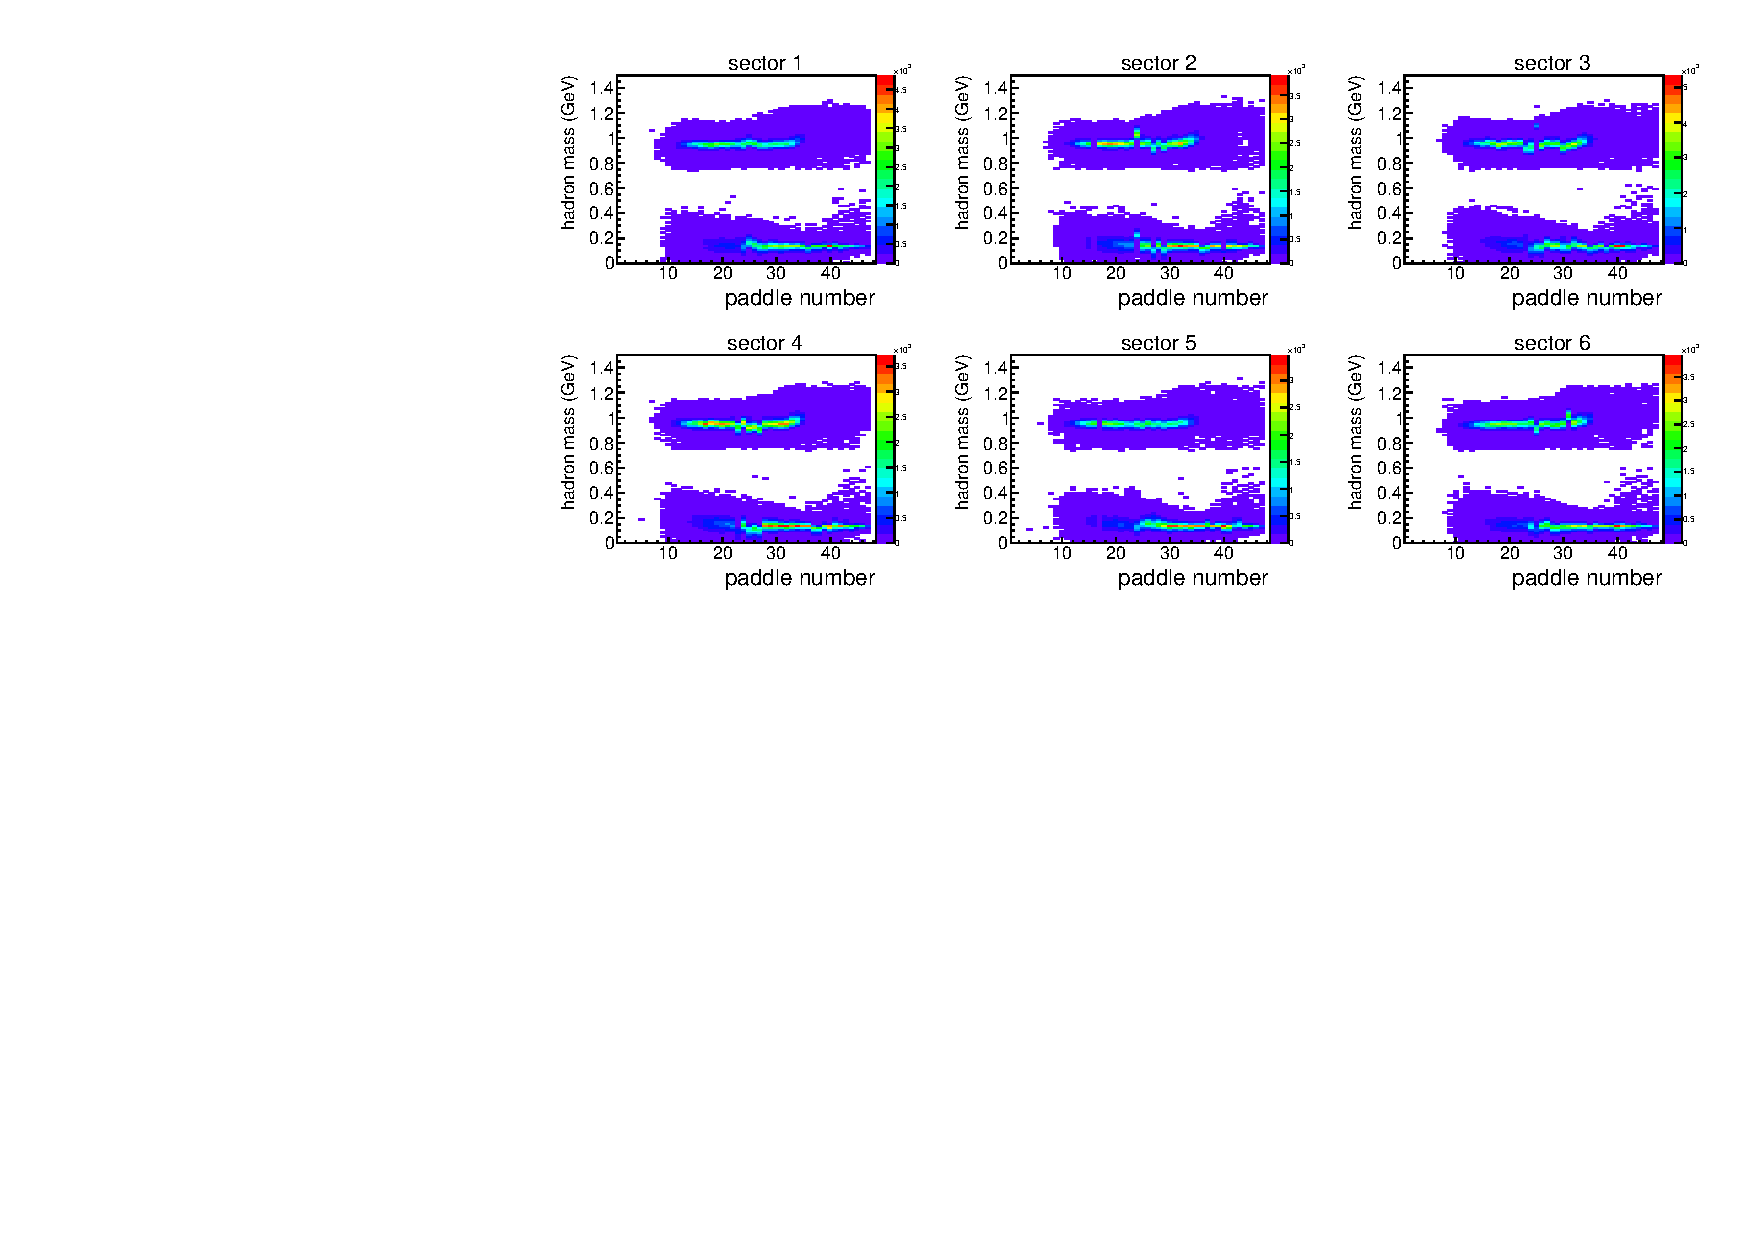
\includegraphics[width=12cm]{mass_no_th_vs_p.pdf}}
\caption{\small  Masses of the protons and $\pi^{+}$ as function of paddle number for six CLAS sectors before $\theta$ vs momentum cuts from Section. 3. \label{mass_no_th_vs_p}} 
\end{center}
\end{figure}  

\begin{figure}
\begin{center} 
\framebox{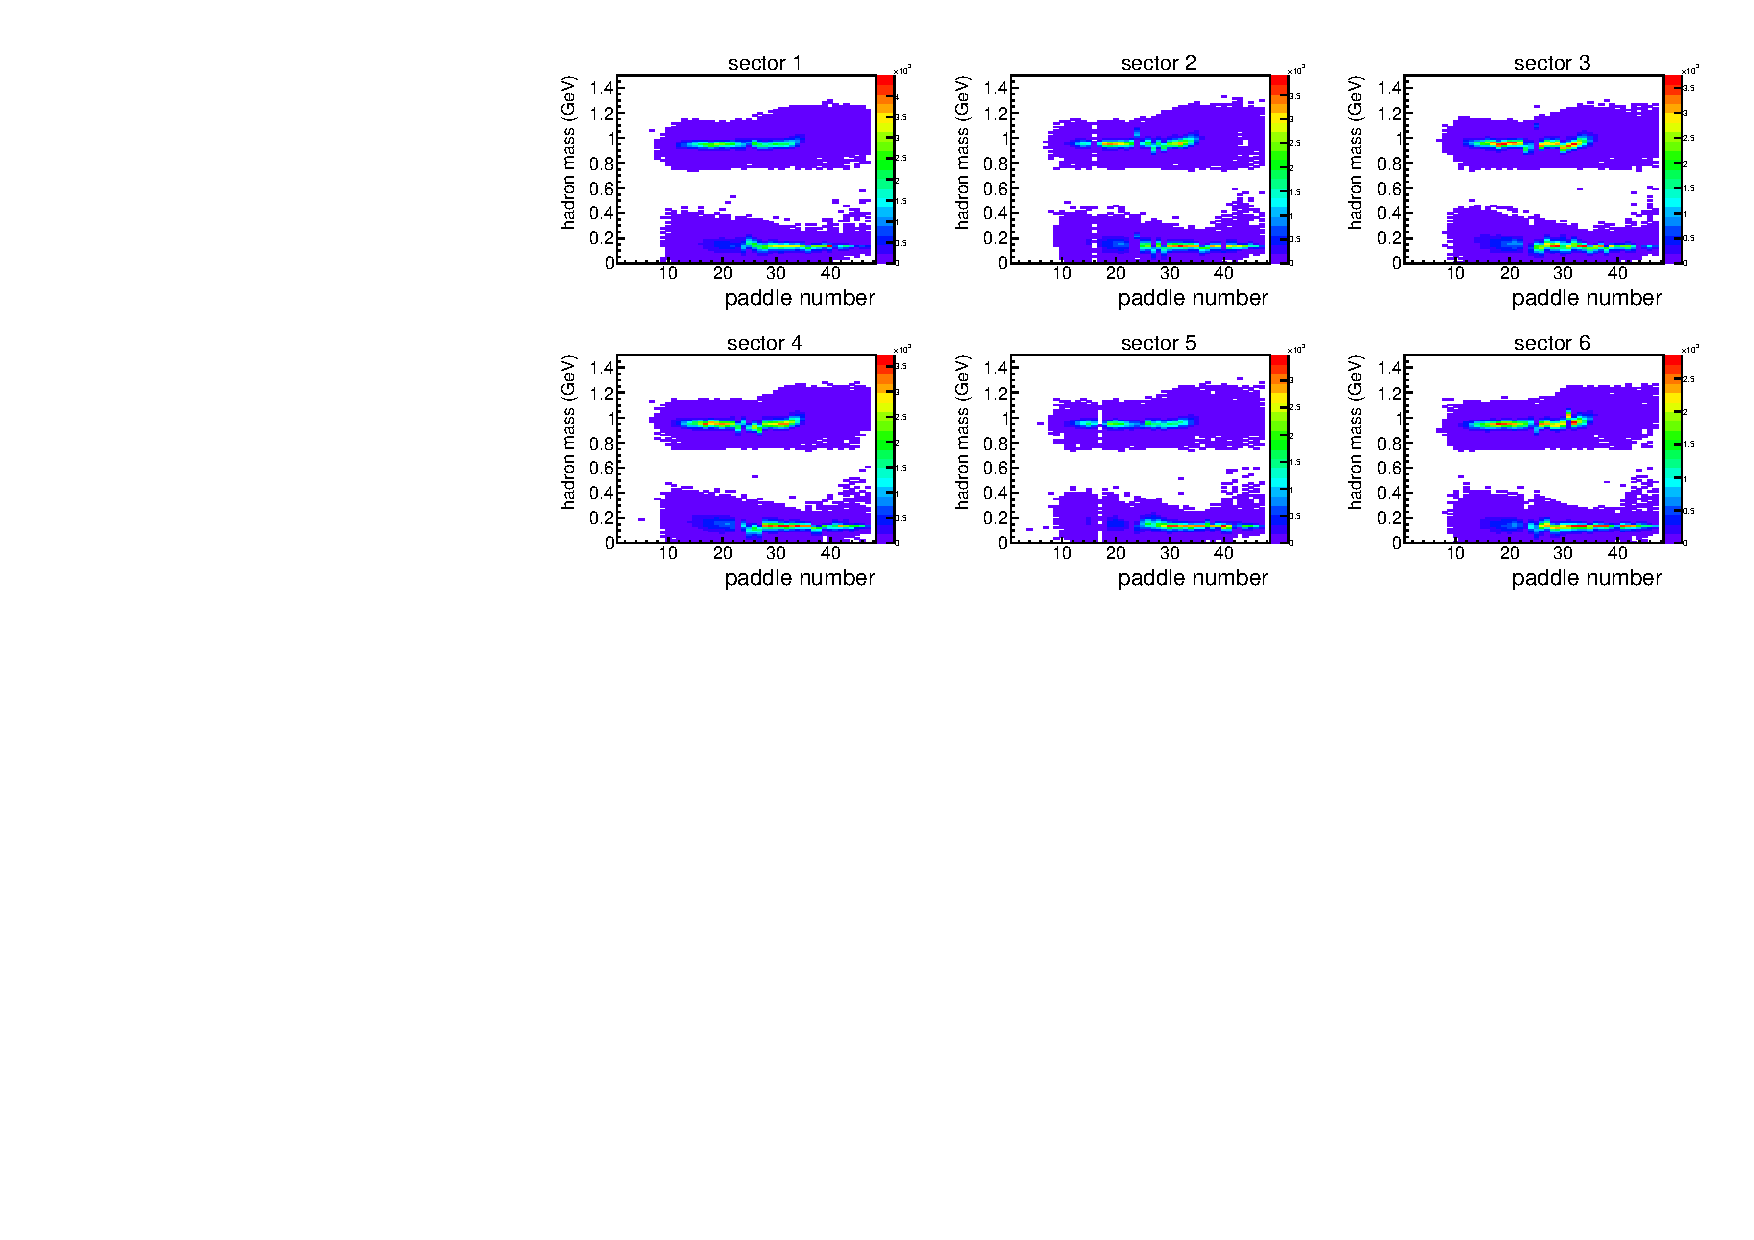
\includegraphics[width=12cm]{mass.pdf}}
\caption{\small  Masses of the protons and $\pi^{+}$ as function of paddle number for six CLAS sectors after $\theta$ vs momentum cuts from Section. 3.  \label{mass}} 
\end{center}
\end{figure}


{\bf 15. Section 2.1.2 -- As you have a liquid-hydrogen target, I am not sure that I 
understand the strong bands beneath the protons for nearly all counters. 
These look like protons where you have identified the wrong RF bunch. How 
are you doing the RF bunch selection? Are you doing it in your analysis code 
or was this done during cooking?}\\[0.5cm] 

RF corrections that were done during the cooking were used. However some problem with timing still remained after the cooking. To solve this problem extra timing corrections were done on levele of the analysis code (see Section. 2.1.3). The strong bands that are seen beneath the protons most likely correspond to the deuterons that are present anyway even in liquid-hydrogen target runs. To check that we superimpose the theoretical curves with deuteron mass assumption (see Fig.~\ref{fig:b_vs_p_positive}) on the $\beta$ vs momentum plots. These bands seem to be strong most likely due to the logarithmic scale. We also checked SEB id for events from these bans and it appears to be equal to 45 that corresponds to the deuteron.\\[0.5cm]  


\begin{figure}[htp]
\begin{center}
\framebox{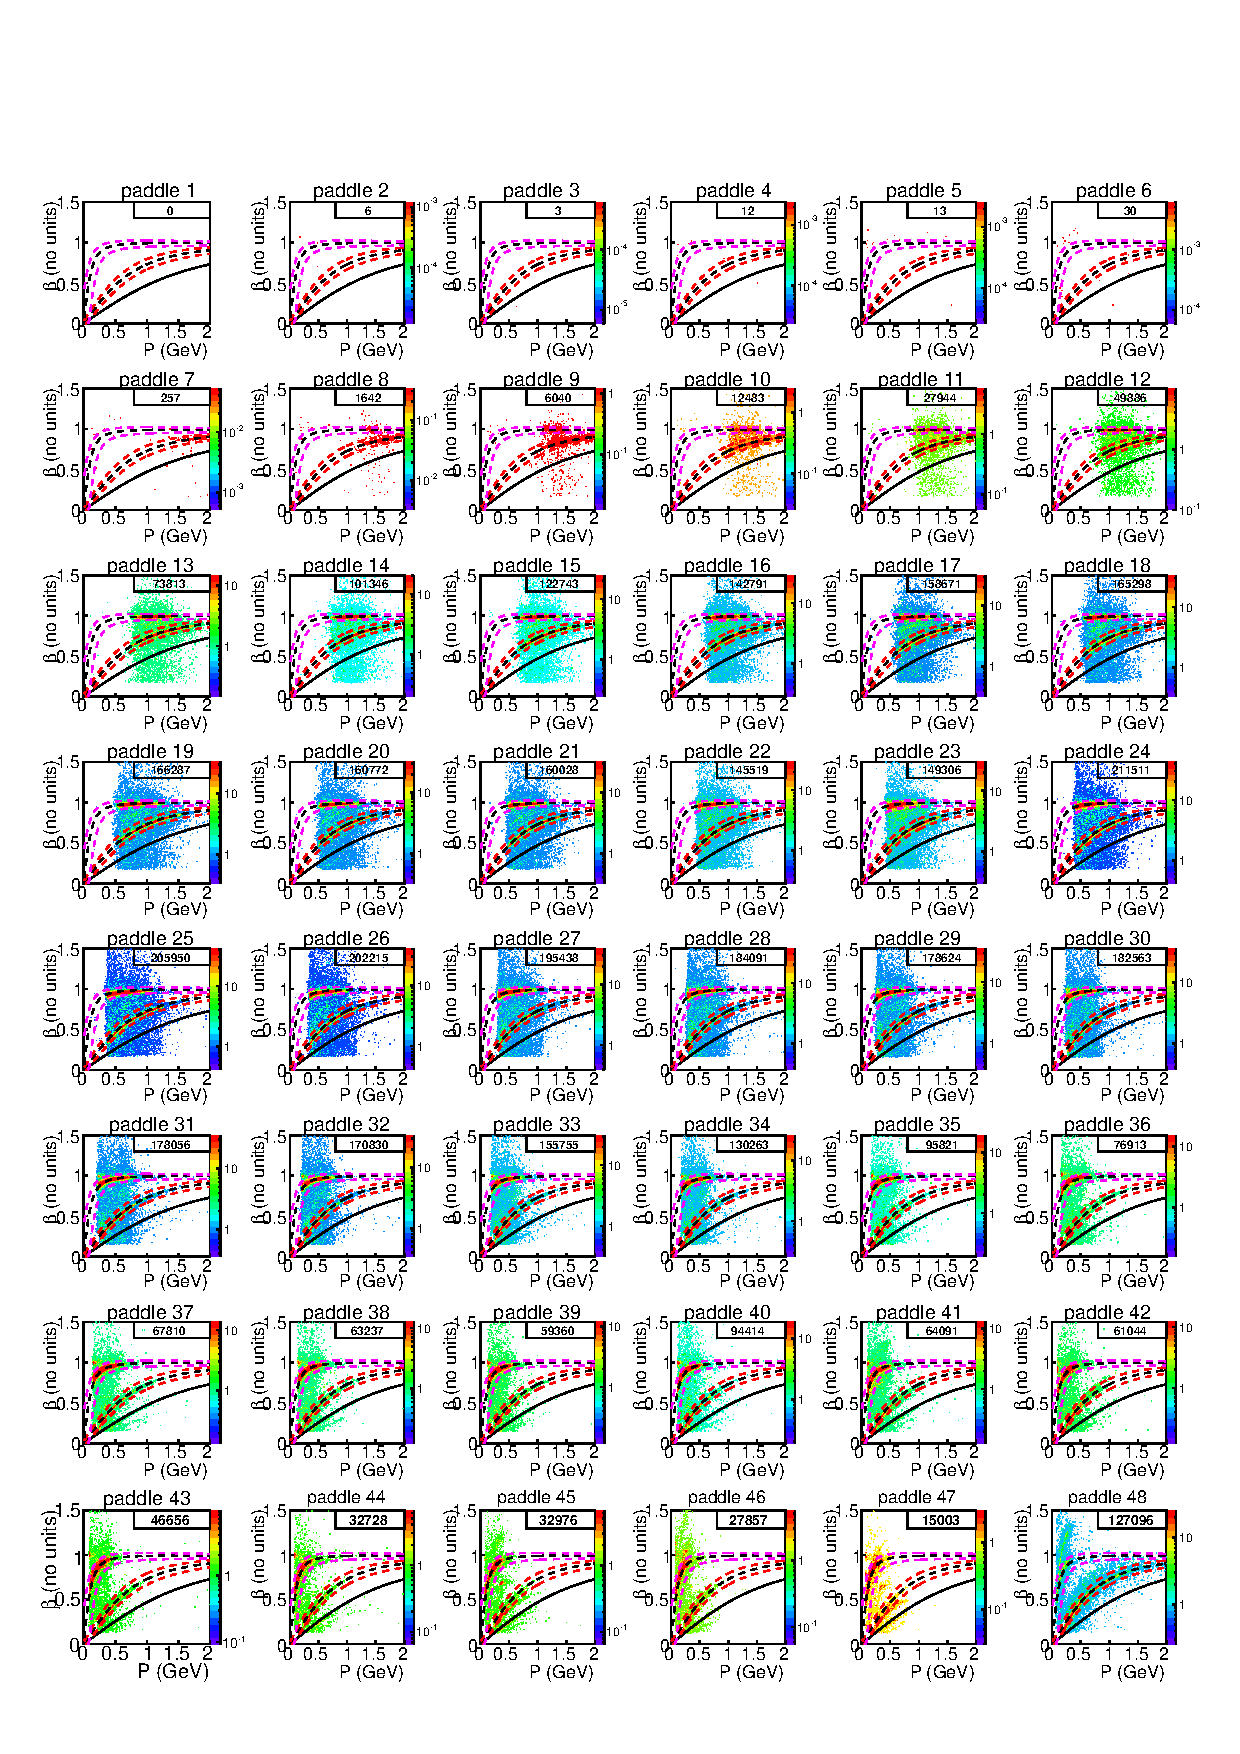
\includegraphics[width=14.5cm]{b_vs_p_deuteron.pdf}}
\caption{\small  $\beta$ versus momentum distributions for positively charged particles for different TOF scintillators in CLAS sector one. Black dashed curves are theoretical under the exact hadron mass assumption~\ref{eq:hadron_hadronmass}. Events between the two purple dashed~\ref{eq:hadron_pioncuts} and two red dashed~\ref{eq:hadron_protoncuts} curves are selected as $\pi^{+}$ and proton candidates, respectively. For scintillators with number greater equal 40 all events laying higher than the upper red dashed curve are assumed as $\pi^{+}$ candidates. Number of events is shown in the right upper corner of each plot. The theoretical curves with deuteron mass assumption are shown by solid black. \label{fig:b_vs_p_positive}} 
\end{center}
\end{figure}

{\bf 16. Your electron momentum correction is developed based on and tested again 
elastic events, which have rather limited momentum coverage. Did you look 
at the effect of the correction on quantities like missing mass $ep \rightarrow ep\pi^{+}X$, $ep \rightarrow ep\pi^{-}X$?}\\[0.5cm] 

Yes, we checked missing mass distributions for the reactions you mentioned above. (see Fig. 3.13). After allcorrections the missing masses appear to be on the right positions for all ranges in $W$ and in good agreement with MC (that does not use this momentum correction procedure).\\[0.5cm]


{\bf 17. You could mention in the text that the elastic peak width is about 9.1 MeV. It would give people an idea about momentum resolution for electrons in e1e.}\\[0.5cm]

The sentence about elastic peak width was added to the Section. 2.2.1\\[0.5cm]

{\bf 18. Section 2.2.1 -- You do not provide any real detail on your momentum 
corrections here. Is Fig. 2.11 made just detecting an inclusive electron? If so, I assume that you are only correcting the electron momentum and assuming 
that there is no mis-measurement of the polar angle? Is this correct?}\\[0.5cm]	 
 The detailed description of the momentum correction procedure is given in reference [27]. It uses the elastic events with proton measured and provides corrections for both electron polar angle and momentum. 
 
 Fig. 2.11 (Fig. 2.12 in the new version) is made with just detecting an inclusive electron to prove that the correction procedure works well.\\[0.5cm]
 
 
{\bf 19. Section 2.2.1 -- It is certainly the case (for the reasons that you mention) that you need to correct the final state particle momenta. However, you correct the electron but ignore the hadrons. This does not make sense.}\\[0.5cm] 
You are right, from what is written in the text it is hard to understand the reason of ignoring the hadron correction. The explanations are presented below and also added to the text of the note.

From reference [27] it is known that momentum corrections are essential only for high-energetic particles. For example for analized dataset ("e1e", beam energy $\sim$ 2 GeV) elastic peak shift from nominal value is about 3 MeV, while for "e1-6" dataset (beam energy $\sim$ 6 GeV) this shift is about 20 MeV. Since in $2\pi$ kinematics hadrons carry only small portion of the system momentum,  the expected momentum  corrections for them are significantly less than for electrons and can be neglected.

Moreover it is known from [27] that momentum corrections are needed for the particles which go at the low angle $\theta$ ($< 35^{o}$).  But with normal direction of the magnetic field the major part of the positevely charged hadrons goes to the backword angles. It also needs to be mentioned that the topology with $\pi^{-}$ missing is the major contributor to the total statistics.

Finally, the fact that the missing masses for all used topologies are on the correct positions signify that the considered level of the momentum corrections seems to be sufficient.\\[0.5cm]
  
{\bf 20. Section 2.2.2 -- Show  $\Delta$ p vs. p to give more information.}\\[0.5cm]

The corresponded plot is Fig.~\ref{delta_p_vs_p}. The example is given for one bin in $\theta$ proton since $\theta$ dependence of the correction is not very pronounced.\\[0.5cm]

\begin{figure}
\begin{center} 
\framebox{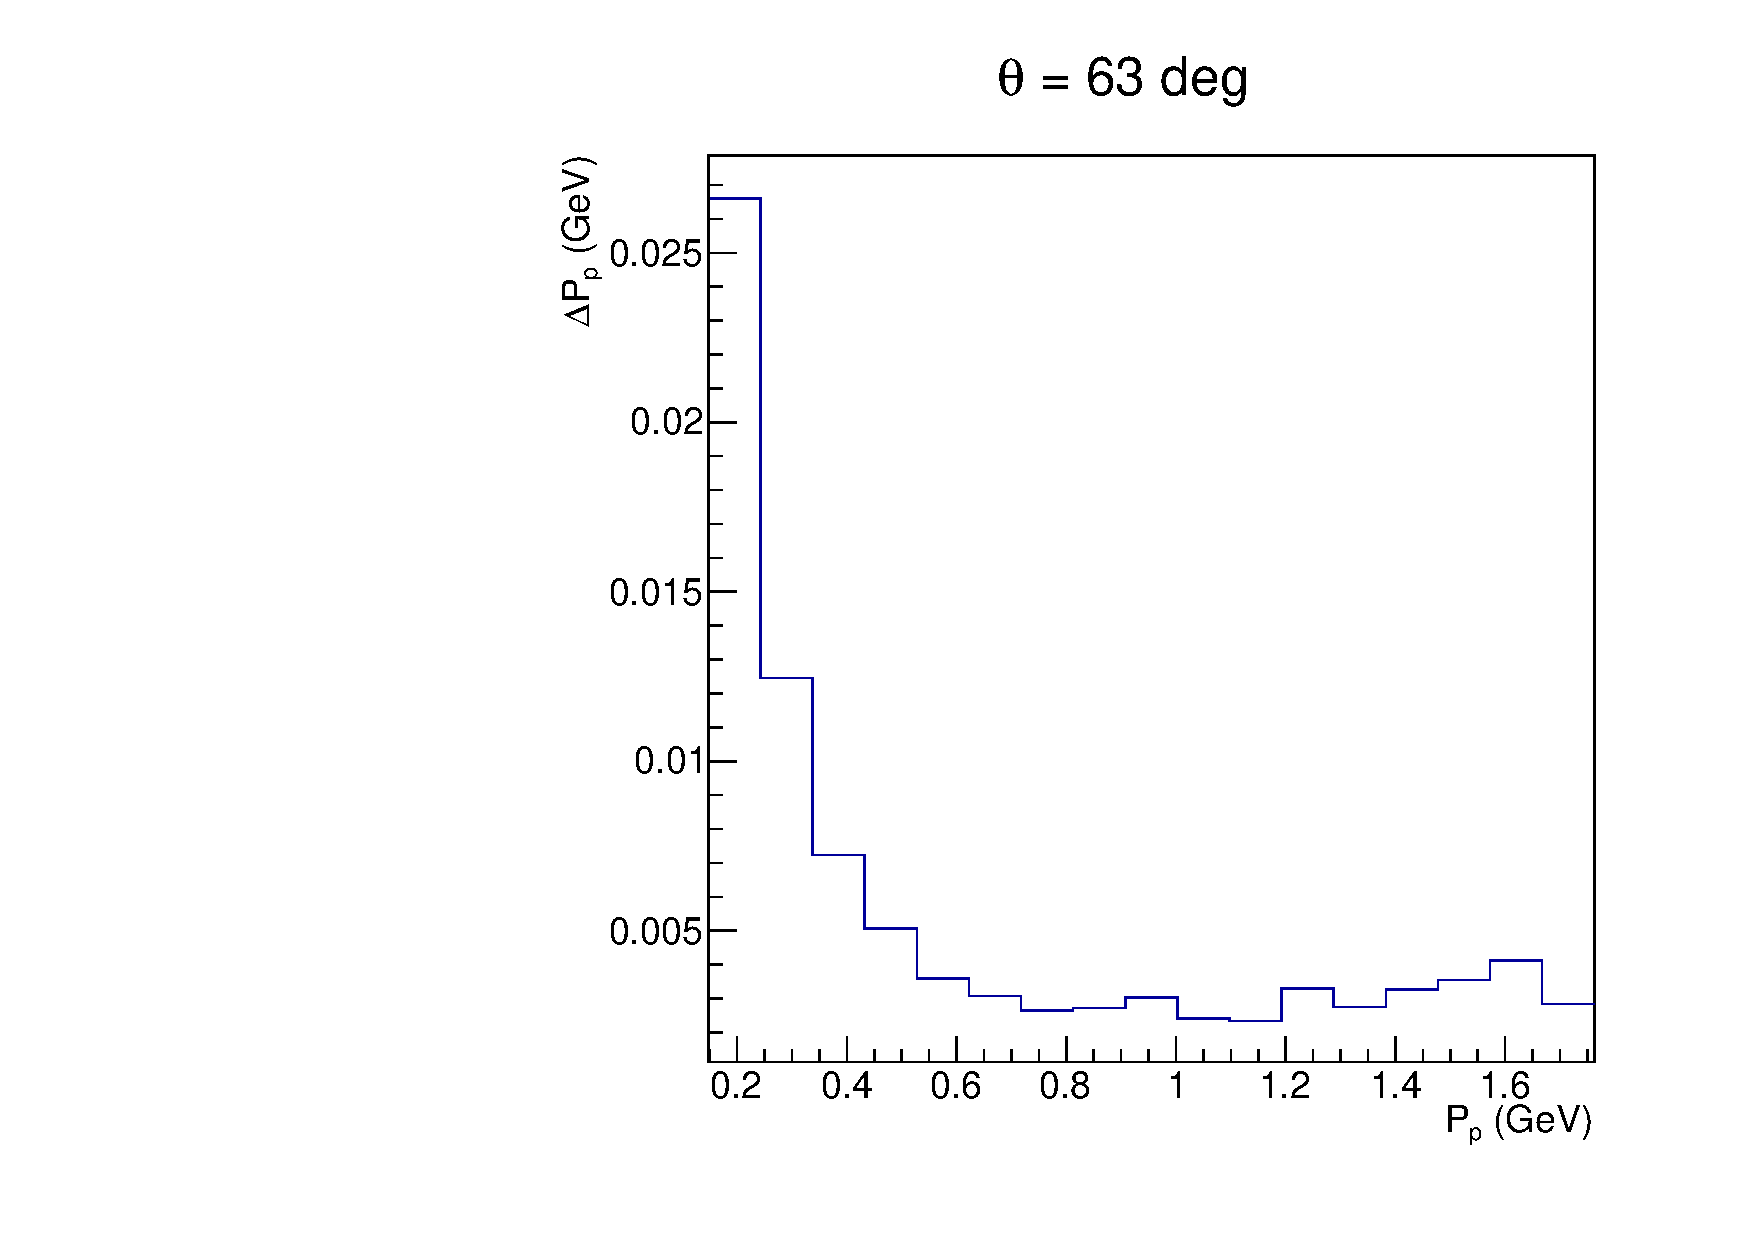
\includegraphics[width=12cm]{proton_eloss/delta_p_vs_p.pdf}}
\caption{\small  The amount of the momentum that protons lose when they move through the detector and target media as a function of the proton momentum. The example is given for one bin in $\theta$ proton.   \label{delta_p_vs_p}} 
\end{center}
\end{figure} 

 
{\bf 21. Hadron ID -- Do you include a minimum hadron momentum cut in your 
analysis? If so, what is it? If not, then I would like to know exactly the theta vs. momentum range covered by all final state particles (actually I would like 
to see this anyway). CLAS was not designed to measure very low momentum 
particles (below a few hundred MeV).}\\[0.5cm]


The minimum hadron momentum cut is not included in the analysis code explicitly. However, after the event selection no hadrons with very low momentum survive. The theta vs. momentum plots for all final state hadrons are given in Figs. 3.4 for $\pi^{-}$, 3.6 for proton, 3.7 for $\pi^{+}$.\\[0.5cm]

{\bf 22. Section 2.2.3 -- Was the e1e target and scattering chamber properly included in GSIM? Is this what you used to determine the correction factor of Fig. 2.14?}\\[0.5cm]

Yes, it was. To prove that $z$ distributions of electrons were plotted for MC and compared with the data (see Fig. 3.12). And yes, MC was used to determine the correction factor of Fig. 2.14 (Fig. 2.15 in the new version).\\[0.5cm] 

{\bf 23. Section 3.1.1, line 410. Do you employ the same fiducial cut for all six sectors? }\\[0.5cm]

Yes, the shape of the fiducial cut is the same for all six sectors.\\[0.5cm] 
  
{\bf 24. Section 3.1.2, line 426. Same for the positive particles.}\\[0.5cm]	

We came that the shape given by equation 3.1.2 (3.1.3 in the new version)  is suitable for all six sectors.\\[0.5cm]

{\bf 25. Section  3.1.1,  line  415,  Figs.  3.4,  3.6,  3.7.  How  do  you  determine  the  shape  of  the  theta  --  momentum  cuts?}\\[0.5cm]

The shape of the theta  --  momentum  cuts was determined in the following way.
Local minimum was found in each 1d slice of 2d theta vs momentum histograms. Then the set of the positions of these minima was fit by certain function. Finally these functions were shifted to the edges of the problematic areas.\\[0.5cm] 

{\bf 26. Section 3.2, line 447. Is it possible that run starts (ends) in the middle of the block? If yes, what do you do with events before first (after last) FC reading in the run?}\\[0.5cm]

To avoid this situation the first and last blocks in each file were removed. The note about that was added in Section 3.2.\\[0.5cm] 

{\bf 27. Page 28. Sec 3.2. What was the length of a "block"?}\\[0.5cm] 

Each "block" corresponds to the time between two FC readouts which happen approximately once in 10 seconds.

{\bf 28. Section 3.3, line 464. Could you elaborate on the vertex correction?}\\[0.5cm]	

The vertex position was taken from DCPB bank where already beam-offset corrected values are stored. In this way good agreement between data and MC was achieved. This information is only used for the cut on $z$ position and is not used in any calculations.\\[0.5cm] 

{\bf 29. Section 3.6, line 516. Section is called "Cuts summary" while fully dedicated to binning and kinematical coverage.}\\[0.5cm]

In the new version of the note the name of Section 3.6 was changed.
Now it is called "Binning and kinematical coverage".

{\bf 30. Fig. 3.8 -- What causes the 10\% shifts seen in this figure? Was there some event noted either in the MCC logbook our the Hall B logbook to point so an explanation?	}\\[0.5cm]

We are not sure about these shifts, most likely they correspond to improper operation of some detector parts. There was a break in the run duration that was connected with Christmas holidays. We suspect that something had changed after the run renewal.\\[0.5cm] 

{\bf 31. Figs. 4.3, 4.4, 4.5 -- What defines  $\alpha =0$? }\\[0.5cm]

The relation 4.1.7 defines $\alpha_{\pi^{-}} =0$ for the second set of variables. This situation corresponds to the vectors $\vec{\gamma}$ and $\vec{\beta}$ shown in Fig. 4.4 to be collinear. In terms of particles directions this means that initial proton is laying in the plane in which all final hadrons are situated. Plus one extra condition that distinguishes $\alpha_{\pi^{-}} = 0$ and $\alpha_{\pi^{-}} = \pi$. If $\pi^{+}$ is toward and final proton is anti-toward the initial proton then $\alpha_{\pi^{-}} = 0$ and vice versa if $\pi^{+}$ is anti-toward and final proton is toward the initial proton then $\alpha_{\pi^{-}} = \pi$. 

For other sets of variables $\alpha$ angle of the corresponded hadron is defined similarly.\\[0.5cm]


{\bf 32. Section 4.2 -- Where does the CC efficiency come in for Eq.(4.2.6)?}\\[0.5cm]

There is no CC efficiency in Eq.(4.2.6) since the correction factor due to the photoelectron cut was applied as a weight for each event. (see the answer to the question six). The clarifying sentence is added to the Section 4.2 of the new version of the analysis note.\\[0.5cm]  

{\bf 33. Eq.(4.2.6) -- As written here, your empty target subtraction form does not make sense. You need to scale the charge in the ratio of $Q_{full}/Q_{empty}$  to get the correct N empty . Include here the values of $Q_{full}$  and $Q_{empty}$  for your good run lists. Also, a statement on how these charges were determined is necessary.}\\[0.5cm]	
  
Eq.(4.2.6) may look a little bit misleading, but it is correct because $Q_{full}$ is moved from the denominator to the numerator. 
The values of $Q_{full}$  and $Q_{empty}$ are given below and also included into the text of analysis note.

\begin{equation}
\begin{split}
Q_{full} & = 5999.64 \; \mu C  \\ \nonumber
Q_{empty} & = 334.603 \; \mu C \nonumber 
\end{split}
\end{equation}

The charges on FC were calculated by summing up charges of all {\em blocks} that passed quality check cuts. See the definition of {\em block} in Section 3.2.\\[0.5cm]


{\bf 34. Section 4.2. What is the relative size of the MC contribution to the statistical uncertainty vs. the yield uncertainty across your phase space? If the yield uncertainty does not totally dominate (as Fig. 4.10 shows), why not just run more MC events until this is the case?  }\\[0.5cm]

The statistical uncertainty is totally dominated by the yield uncertainty. In Fig. 4.10 the relative efficiency error is given in 7D kinematical cell. As it seen from the  plot there are a lot of events reconstructed, while for the data we typically have just one event in multi-dimensional cell. Our MC statistics is higher than in all previous $2\pi$ analyses and exceeds data statistics more than 1500 times.\\[0.5cm]

{\bf 35. Fig. 4.11 $\alpha_{\pi^{-}}$ distribution consistently does not match the data. Any comment?}\\[0.5cm]

The $\alpha_{\pi^{-}}$ and $\alpha_{\pi^{+}}$ cross sections obtained from new $2\pi$ event generator and shown by green curves in Fig. 4.11 were occasionally swapped around. This mistake is corrected in the new version of the analysis note. Thank you.  


%The green curves in Fig. 4.10 are not a model fit, they show the cross section from new $2\pi$ EG that was used to fill out empty cells. The cross sections from new $2\pi$ EG are obtained from JM model predictions in those regions where they exist.  In the regions where JM model predictions 	do not exist the new EG emploes a special interpolation/extrapolation procedure (see https://userweb.jlab.org/$\sim$skorodum/pictures/secure/docs/clas\_col\_meet\_skor.pdf). For the bin ($W = 1.6375$~GeV, $Q^{2} = 0.525$~GeV$^{2}$) shown in Fig. 4.10 there are no model predictions, so the green curves in Fig. 4.10 correspond to the best cross section approximation that available up to now.\\[0.5cm] 


{\bf 36. Fig. 4.11. In all three plots, in the cross section over  $\alpha\pi^{+}$  there is a significant difference between "unfilled" and model cross section around 180 degrees. Naively I would expect that to lead to a significant difference between "filled" and "unfilled" cross section (similar to what you have for cross section over $\theta_{\pi^{-}}$  at low/high angles) but there is very small difference. Could you please comment.}\\[0.5cm] 

There was a mistake, see the answer to the question 35.

%The difference between "filled" and "unfilled" cross sections is determined by the amount of empty multi-dimensional cells that contribute into the particular point in one-dimensional distribution. Due to the CLAS acceptance this amount is maximal at the forward and backward $\theta$ angles being small in other areas. If the amount of empty cells is relatively small the difference between "filled" and "unfilled" cross section is also small even if the EG cross section (green curves in Fig. 4.11) differs from the experimantal one significantly.\\[0.5cm]

{\bf 37. Section 4.6 -- I need more detail on exactly how you combine the events for the different topologies. There should be only three topologies (please 
confirm): $e p \rightarrow e' p' \pi^{-} X$, $e p \rightarrow e' p' \pi^{+} X$, and $e p \rightarrow \pi^{+} \pi^{-} X$. How do you ensure there 
is no double counting? How do you account for the different CLAS 
acceptances? I think that it would be important to compare cross sections 
directly for the different topologies to see if there is agreement within your 
quoted systematics.}\\[0.5cm]

One can distinguish four topologies:
\begin{itemize}
\item $e p \rightarrow e' p' \pi^{+} X$
\item $e p \rightarrow e' p' \pi^{-} X$
\item $e p \rightarrow e' \pi^{+} \pi^{-} X$
\item $e p \rightarrow e' p \pi^{+} \pi^{-} X$
\end{itemize} 
These topologies are defined in a way they do not overlap. For example the topology $e p \rightarrow e' p' \pi^{+} X$ requires the presence of $e'$, $p'$ and $\pi^{+}$ candidates and absence of $\pi^{-}$ candidates, avoiding in this way double counting. This explanation was added to the Section 3.4. 

The explanation of the topologies combination and corresponded CLAS acceptance calculation is given in Section 4.6. Our main topology is $e p \rightarrow e' p' \pi^{+} X$, it contains 70\% of statistics. Due to the run conditions all other topologies are dominated by the kinematical cells with zero acceptance and the cross sections obtained for these topologies individually are very model dependent and their direct comparison is not informative. So, we decided to compare the cross sections obtained for various ways of topology combinations (see Fig. 4.11).\\[0.5cm] 


{\bf 38. Section 5, line 848. From previous Section I've got an impression you have a model, which you use to generate events. Isn't it better to use a model to estimate the bin centering correction?}\\[0.5cm]  	

Actually it is not a model it is just the cross section from new $2\pi$ EG. 

The green curves in Fig. 4.10 are not a model fit, they show the cross section from new $2\pi$ EG that was used to fill out empty cells. The cross sections from new $2\pi$ EG are obtained from JM model predictions in those regions where they exist.  In the regions where JM model predictions 	do not exist the new EG emploes a special interpolation/extrapolation procedure (see https://userweb.jlab.org/$\sim$skorodum/pictures/secure/docs/clas\_col\_meet\_skor.pdf). 

So, we decided that it is better to use the data cross section shape for the bin centering correction.\\[0.5cm]

{\bf 39. Section 6.1. Is the elastic cross section you present measured with electron detection only?}\\[0.5cm]

Yes, only the detection of the scattered electron was required.\\[0.5cm]

{\bf 40.  Page 51. Formula 4.2.14 
It is not a correct way to calculate statistical errors for Monte Carlo 
simulation, since Ngen and Nrec are not independent variables.  
As I remember, if eff = Nrec/Ngen, then  
\textbackslash sigma(eff)/eff = \textbackslash sqrt$\{$Ngen-Nrec$\}$/Nrec.	
}\\[0.5cm]

You are right. Now to calculate statistical errors for Monte Carlo 
simulation the following formula is used:
$$
\frac{\sigma_{eff}}{eff} = \sqrt{\frac{N_{gen}-N_{rec}}{N_{rec}N_{gen}}}
$$
The explanation was added to the Section 4.2. All the cross sections and errors in the analysis note were recalculated.\\[0.5cm]

{\bf 41. Section 6.4 -- Do you assign the average/typical value as the systematic for all 
bins or what you determine for each individual bin? Please provide a plot of 
the kinematic and statistical dependence of your systematic uncertainties. }\\[0.5cm] 

The systematical uncertanties due to the different ways of combining topologies and due to the integration over different final hadron variables were determined in each bin in $W$ and $Q^{2}$ individually (see Fig.6.2). While the systematical uncertanties due to the normalization, electron id, and
 electron detection efficiency and due ti the radiative corrections are assigned globally. In the Table 6.1 the typical values of the systematical uncertanties in $W$ and $Q^{2}$ bin are given. The explanation is added to the text.\\[0.5cm]

{\bf 42. Section 6.4 Do you have any estimate on the systematic error from hadron identification? }\\[0.5cm] 

We assume that error due to the hadron identification is already taken into account by the error due to the different ways of combining topologies since in various topologies different hadrons are registered and therefore different hadron selections are used. So, to avoid overestimation of the systematical uncertainty due to including twice the same effects we decide not to assign any specific error to the hadron identification.\\[0.5cm]

{\bf 43. Section 6.4. What is you estimation of the total error? }\\[0.5cm] 

The total cross section uncertainty (both statistical and
systematical ones summed up in quadrature) is shown by the hatched red areas in Fig. 6.2.\\[0.5cm]

{\bf 44. Fig. 7.1 -- Does this include statistical uncertainties on the points?}\\[0.5cm]	

Yes, it does, but due to the small value of the statistical error they are invisible under the symbols.\\[0.5cm]

{\bf 45. Page 59. line 856. Can you estimate quantitatively the asymmetry of alpha distributions and compare it with the errors in Table 6.1. I think it is a good 
way to check the obtained uncertainty of the cross section.}\\[0.5cm]
  
\end{document}


